\chapter{Budowa aplikacji} 
%============================================================================================================================
% Glowna petla
%============================================================================================================================

\section{Główna pętla}
\lhead{Rozdział 2. \emph{Główna pętla}}

W grach komputerowych często wykorzystywane jest tzw. programowanie sterowane zdarzeniami. Polega ono na umieszczeniu w aplikacji głównej pętli, w której to cyklicznie będzie się odbywać obsługa zdarzeń (np. naciśniecie klawisza ), aktualizacja gry oraz rysowanie. Sama kolejność tych elementów nie odgrywa większej roli, warto natomiast zwrócić uwagę na to, że po zatrzymaniu pętli następuje przygotowanie aplikacji do wyłączenia. W przypadku Astro Rush po wyjściu z głównej pętli zatrzymywany jest kontekst graficzny SDL-a, zwalniane są wszystkie zajęte zasoby, i następuje wyłączenie gry. Pętla taka najczęściej implementowana jest jako while, którego zakończeniem steruje flaga wyjścia. Przy każdym obiegu pętli wartość tej flagi wyciągana jest z klasy Game, która to decyduje kiedy należy zakończyć działanie aplikacji. 

\begin{figure}[h]
    \centering
    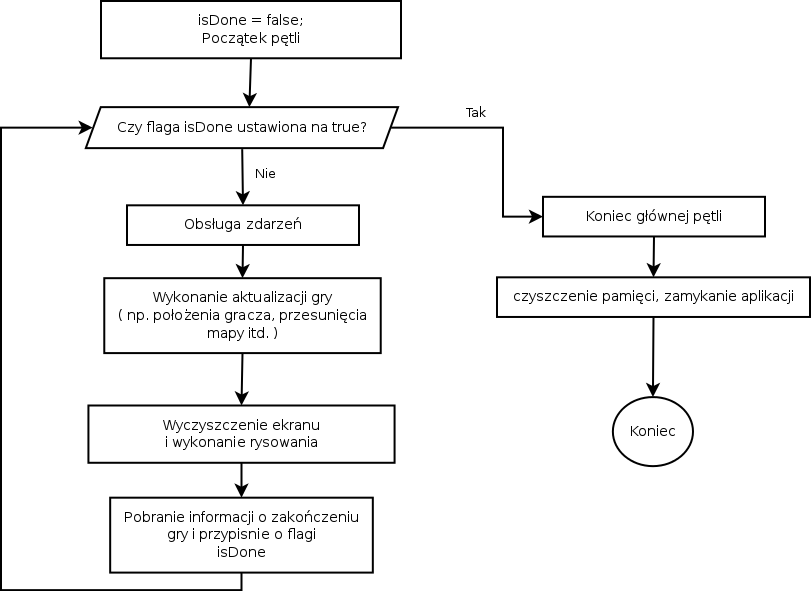
\includegraphics[width=0.8\textwidth,natwidth=410,natheight=142]{./Pictures/main_loop.png}
    \caption{Schemat działania głównej pętli}
\end{figure}

Pętla stanowi najważniejszy element większości gier, to od niej zależy czy gra będzie działać tak samo na urządzeniach różniących się wydajnością. W projekcie pętla jest dość prosta i oprócz typowych elementów typu aktualizacja, rysowanie, obsługa zdarzeń, uwzględnia jedynie sytuacje w której całość obliczeń i rysowań odbywa się zbyt szybko i należy wykonać opóźnienie. Taki problem może się pojawić na szybszych urządzeniach na których gra działała by zbyt szybko. W przypadku bardziej złożonej aplikacji można także uwzględnić sytuacje odwrotną, kiedy to ostatnia aktualizacja stanu gry odbywała się zbyt wolno i w następnym obiegu pętli należy wykonać aktualizacje kilkukrotnie żeby zapobiec braku płynności w renderowanym obrazie. Taka sytuacja jednak w grze Astro Rush nie powinna mieć miejsca z racji tego, iż jest jest to gra z grafiką dwuwymiarowa i występują w niej proste obliczenia matematyczne.


%============================================================================================================================
% Mapa kafelkowa
%============================================================================================================================
\section{Mapa w grze}

\lhead{Rozdział 2. \emph{Mapa kafelkowa}}
\subsection{Mapa kafelkowa}
Mapa kafelkowa (ang. tiled map) jest jedną z podstawowych technik przy tworzeniu gier z grafiką dwuwymiarową. Technika ta polega na podziale świata dostępnego w grze na fragmenty (tzw. kafelki ) o tych samych rozmiarach. Najczęściej są to kwadraty, którym przypisujemy odpowiednie identyfikatory grafik. Tak utworzona mapa przechowywana jest w postaci dwuwymiarowej macierzy w osobnym pliku na dysku, i jest wczytywana podczas startu aplikacji w osobnym wątku. Macierz składająca się wyłącznie z cyfr (typu short żeby dodatkowo oszczędzić pamięć) zajmuje o wiele mniej pamięci w przeciwieństwie do rozwiązania w którym  z dysku wczytywana jest cała mapa w postaci jednej grafiki. Na podstawie tej macierzy rysowana jest mapa widoczna na ekranie. 

Z racji tego, że gracz ciągle wędruje prze mapę, ta cały czas jest przesuwana, a dokładniej  to inkrementowany jest indeks kolumny w macierzy kafelków od której zaczynamy rysowanie. Kolumna o takim indeksie rysowana jest na ekranie jako pierwsza z lewej strony, następnie rysowane są obok (po prawej stronie) kolejne kolumny aż do momentu w którym mapa pokrywa cały ekran.
Kolumna od której zaczyna się rysować od lewego brzegu ekranu przesunięta jest w lewo o pewien offset, który zwiększany jest podczas biegu gracza do przodu. Offset ten sprawia, że współrzędna na osi X skrajnej kolumny zostaje przesunięta w lewo po za ekran, tak, że widoczny jest tylko fragment kolumny na ekranie. Przejście do następnej kolumny następuje w momencie kiedy skrajna kolumna znajduje się całkiem po za ekranem. Dzięki zastosowaniu takiego algorytmu następuje płynne przesuwanie mapy, bez widocznych przeskoków pomiędzy kolejnymi kolumnami.

\begin{figure}[h]
    \centering
    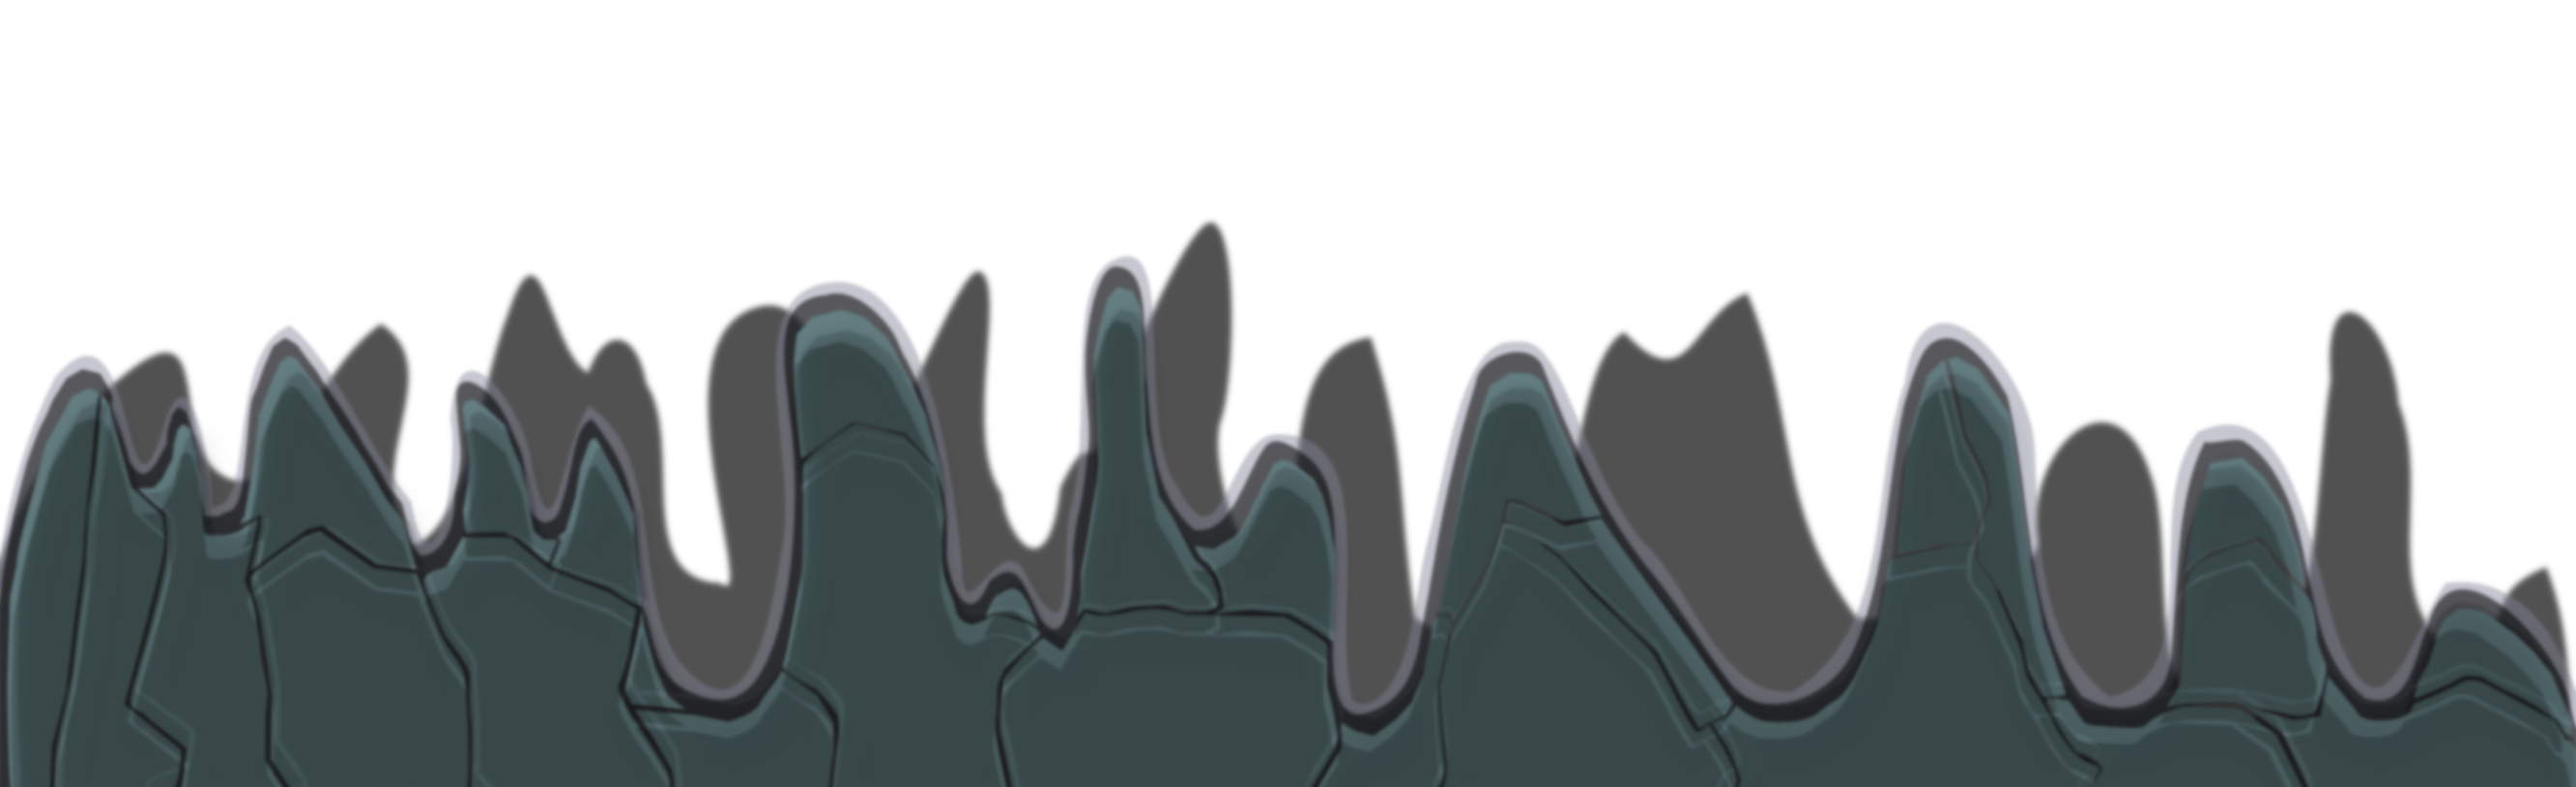
\includegraphics[width=0.8\textwidth,natwidth=800,natheight=160]{./Pictures/back.png}
    \caption{Przewijane tło wyświetlane w grze}
\end{figure}

Warto wspomnieć o tle w grze. Tłem mapy jest grafika wykonana w programie Inkscape, przedstawiająca kosmos. Wymiary tej grafiki to 1920 px na 1080 px, w przypadku uruchomienia gry na mniejszej rozdzielczości obraz zostaje przeskalowany, natomiast większa rozdzielczość ( 1920x1080 to popularnie nazywa rozdzielczość HD ) nie jest dopuszczalna w aplikacji i program zakończy się z informacją, że taka rozdzielczość nie jest wspierana. Ograniczenie takie powstało w celu zapewnienia jednolitego wyglądu na różnych wielkościach monitorów. Dolną graniczną rozdzielczości z jaką może pracować program jest 800 na 600. Wymiary te są zaszyte w kodzie źródłowym jako stałe, przez co nie mogą być modyfikowane przez potencjalnego użytkownika któremu zostanie dostarczona aplikacja. W celu nadania większej atrakcyjności wyświetlane jest drugie tło składające się ze skał obcej planety. 
Tło te przesuwa się w tym samym kierunku co mapa, jednak z inną prędkością żeby nadać
większej atrakcyjności wyświetlanemu obrazowi. Szerokość grafiki to ponad 2500 px, jednak jest to zbyt mało żeby skały mogły się przewijać przez cały czas trwania rozrywki, dlatego też wyświetlanie tego tła ulega zapętleniu, i kiedy na ekranie pojawia się brzeg grafiki, wtedy zaraz za nim pokazuje się następny obrazek tła ryzowany od początku. Dzięki czemu zachowana jest ciągłość i płynność wyświetlanej grafiki. 
 

%============================================================================================================================
% Edytor leveli
%============================================================================================================================
\subsection{Edytor mapy}
\lhead{Rozdział 2. \emph{Edytor mapy}}
Opisana w poprzednim podrozdziale macierz kafelków w grze Astro Rush ma wymiary: 30000 x 15. Stąd też pojawił się problem edycji tak dużej ilości danych. Zmiana poszczególnych wpisów ręcznie nie wchodziła w grę, dlatego też powstała dodatkowa aplikacja do edycji mapy. W wizualny sposób, z wykorzystaniem jedynie myszy można w niej stworzyć w kilkanaście minut całą mapę, rozmieszczając na niej dostępne rodzaje kafelków. Edytor umożliwia także wczytanie stworzonej wcześniej mapy i jej edycje. Aplikacja została napisana z wykorzystaniem biblioteki Qt udostępnionej na licencji LGPL. Biblioteka ta jest zestawem przenośnych narzędzi do tworzenia między innymi interfejsu użytkownika, obsługi sieci, grafiki trójwymiarowej (OpenGL), plików i wielu innych. 


\begin{figure}[h]
    \centering
    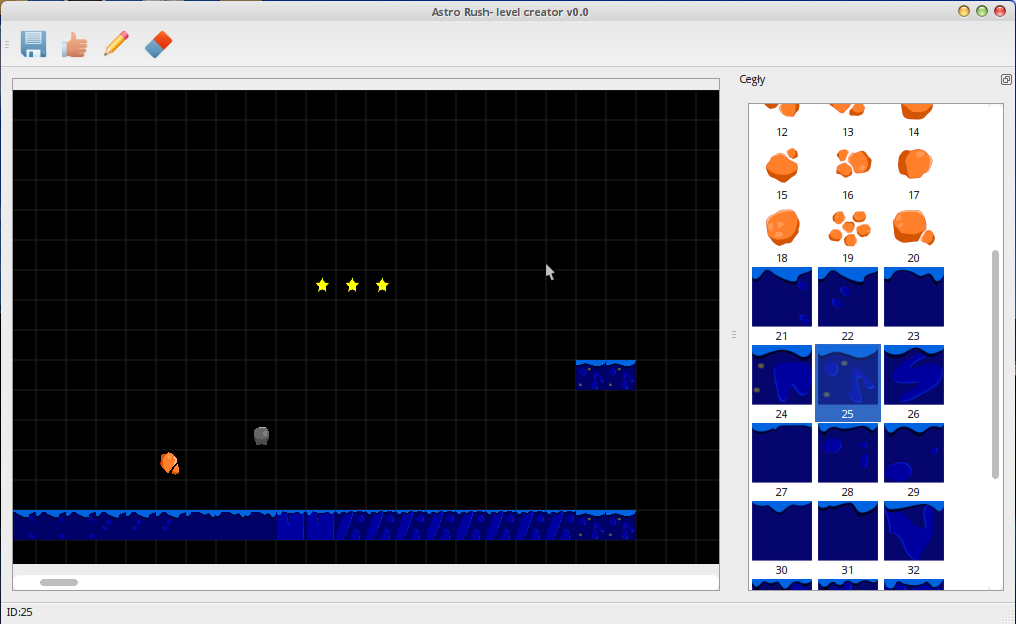
\includegraphics[width=0.8\textwidth,natwidth=800,natheight=160]{./Pictures/designer.png}
    \caption{Edytor mapy podczas pracy}
\end{figure}

Edytor mapy wyświetla całą planszę w postaci siatki na której naniesione są kafelki. Poprzez kliknięci w daną komórkę możemy zmienić rodzaj kafelka, który w danym miejscu ma się wyświetlić, bądź też wyczyścić daną komórkę. Do pliku zapisywane są tylko numery odpowiadającym poszczególnym kafelkom, na bazie których gra rozpoznaje jaką grafikę w danym miejscu wstawić. Numeracja kafelków rozpoczyna się od 0, natomiast wartość -1 oznacza, że w danym miejscu nie ma kafelka i taki fragment nie jest rysowany. Edytor jest aplikacją bardzo prostą, wszelkie jego modyfikacje np. dodanie nowego rodzaju kafelka wymaga ręcznych zmian w kodzie programu, jednak na potrzeby pracy takie rozwiązanie okazało się wystarczające.

%============================================================================================================================
% Uruchamianie aplikacji
%============================================================================================================================
\section{Uruchamianie aplikacji}
\lhead{Rozdział 2. \emph{Uruchamianie aplikacji}}
Aplikacje takie jak gry wymagają do pracy zewnętrznych zasobów które są przechowywane na dysku. Mogą to być grafiki, dźwięki, czcionki. Wraz ze wzrostem ilości materiałów jakie muszą być załadowane do aplikacji przy jej starcie rośnie też czas oczekiwania gracza na to aż aplikacja będzie gotowa do pracy. Dlatego też wczytywanie zasobów, oraz inne czynności które trwają długo są wykonywane podczas uruchamiania, a użytkownikowi prezentowany jest w tym czasie ekran powitalny (ang. Splash screen). W grze Astro Rush taki ekran również jest prezentowany. Pokazuje się na nim również pasek postępu obrazujący ile czasu pozostało jeszcze do uruchomienia właściwej części aplikacji. Żeby samo rysowanie ekranu powitalnego odbywało się płynnie wczytywanie danych z dysku odbywa się w osobnym wątku.

\begin{figure}[h]
    \centering
    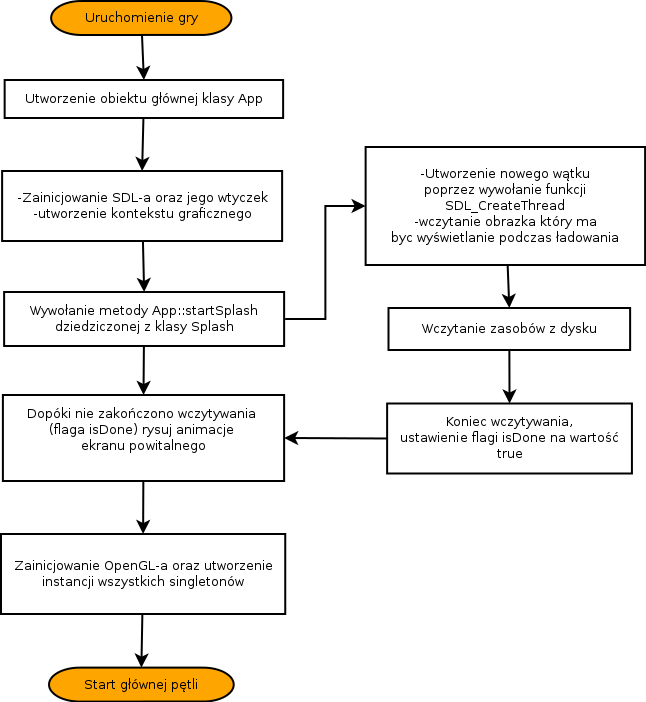
\includegraphics[width=0.8\textwidth,natwidth=800,natheight=152]{./Pictures/splash.png}
    \caption{Schemat uruchamiania gry}
\end{figure}

Wielowątkowość w projekcie jest możliwa dzięki wykorzystaniu specjalnej funkcji z biblioteki SDL. Funkcja SDL\_CreateThread przyjmująca jako argument wskaźnik do funkcji tworzy nowy wątek w którym zostaje uruchomiona ta funkcja. W funkcji takiej zostało umieszczone wczytywanie wszystkich zasobów z dysku. W momencie kiedy funkcja wczyta wszystkie dane, wtedy ustawi flagę oznaczającą zakończenie ładowania na wartość True. Zmiana wartości tej flagi spowoduje zakończenie wyświetlania ekranu powitalnego i uruchomi główną pętle gry. Cała funkcjonalność związana z ekranem powitalnym została umieszczona w osobnej klasie Splash która jest dziedziczona prze główną klasę aplikacji - App. Dzięki takiej implementacji klasa App zajmuję się jedynie inicjowaniem bibliotek, oraz obsługą głównej pętli. 

Należy wspomnieć ile miejsca zajmują omawiane zasoby na dysku. W przypadku  dźwięków jest to około 10 MB, grafika to 3 MB, a sam plik z mapą to 1.3 MB. Na wczytanie takich ilości danych w zależności od sprzętu może być potrzebne nawet do kilku sekund.

%============================================================================================================================
% Przyjęte konwencje, logowanie i obsługa błedów
%============================================================================================================================
\section{Przyjęte konwencje, logowanie i obsługa błędów}
\lhead{Rozdział 2. \emph{Przyjęte konwencje, logowanie i obsługa błędów}}
W fazie analizy projektu zostały przyjęte pewne konwencje które na celu miały przyśpieszyć proces usuwania błędów w kodzie, zapewnić jego czytelność i wysoki poziom. Dodatkowo zostały wprowadzone pewne mechanizmy które miały uspójnić projekt, zostanie to przybliżone w tym rozdziale. 


Nazwy metod oraz pól w aplikacji zostały w większości przypadku zapisane w formie ,,camelCase``, czyli notacji polegającej na pisaniu nazwy składającej się z kilku wyrazów łącznie zaczynając każdy kolejny wyraz z dużej litery. Wyjątek stanowi pierwsza litera z nazwy, która jest małą ( w przeciwieństwie do notacji PascalCase gdzie początek nazwy też jest pisany z dużej litery ). Dodatkowo przyjętą konwencją było pisanie przy nazwach pól litery ,,p`` na początku, bądź też ,,is`` w przypadku zmiennych logicznych. Taki zapis pozwala odróżnić nazwy funkcji od pól. Akcesory do pól prywatnych są nazywane z konwencją przyjętą w języku Java tzn. z przedrostkami get, set, is. Zmienne stałe pisane są drukowanymi literami, a odstępy między wyrazami w takiej nazwie stanowi tzw. ``podłoga,,.

W celu zachowania wysokiej jakości kodu w programie nie są używane takie elementy języka jak skoki goto, zmienne globalne (z wyjątkiem stałych), zaprzyjaźnianie klas. Same klasy natomiast są częściowo opisane za pomocą komentarzy doxygena.

Kwestia dołączania bibliotek do poszczególnych plików źródłowych została rozwiązana za pomocą umieszczenia wszystkich importów bibliotek (ang.include) w jedynym wspólnym pliku, dzięki czemu nie był potrzeby dołączania do każdego pliku np. biblioteki Lua. Plik z potrzebnymi importami to Headers.hpp. Dodatkowo w pliku tym zdefiniowane zostały stałe globalne używane w aplikacji, a nie podlegające modyfikacji z poziomu skryptów Lua np, szybkość biegu gracza. Plik ten dodatkowo zawiera przestrzeń nazw GameSpace zawierającą enumeratory używane np.  do określenia rozmiaru czcionki wypisywanego na ekranie tekstu.

W aplikacji w przypadku błędów krytycznych, w przypadku których aplikacja ma zakończyć działa natychmiast zostaje wyrzucony wyjątek z dowolnego miejsca w aplikacji. Wszystkie nie złapane wyjątki są obsługiwane i logowane w funkcji main. W celu ujednolicenia rzucanych wyjątków wyrzucenie wyjątku zawsze ma następujący wygląd: throw std::runtime\_error(<nazwa\_klasy>::<nazwa\_metody>). Gdzie przed wyrzuceniem wyjątku logowane jest co się dokładnie co stało. W main po złapaniu wyjątku logowana jest treść wyjątku, czyli nazwa metody z której został wyrzucony, następnie zostaje usunięty obiekt klasy App i zwrócony kod błędu EXIT\_FAILURE.
 
W celu ujednolicenenia mechanizmu logowania została utworzona klasa Logger, która posiada 
zestaw funkcji wypisującyhc na ekranie komunikat z odpowiednim priorytetem (DEBUG, INFO, WARRING, ERROR, CRITICAL, FATAL ). Z tym, że funkcja wypisująca w informacje z priorytetem debug wypisze komunikat tylko wtedy kiedy zdefiniowana jest stała DEBUG. Klasa ta posiada dodatkowo pole na nazwę klasy, która używana jest do logowania, pole te może zostać ustawione za pomocą konstruktora w klasie która rozszerza klasę Logger. Informacja z nazwą klasy dopisywana jest do każdego użycia loggera, dzięki czemu łatwiej odnaleźć w logach przyczynę błędu. Takie rozwiązanie na potrzeby tak małego projektu okazało się wystarczające, w przypadku większych projektów zdecydowanie lepszym pomysłem może okazać się użycie dodatkowej biblioteki np. log4c (dla języka C++ jest to odpowiednik znanej z Javy biblioteki log4j). 

Warto wspomnieć także o tym, że duża część klas miała w założeniu używać tych samych elementów, pozwalających wypisywać tekst na ekranie, rysować grafikę, oraz mieć dostęp do takich danych jak np. wymiary ekranu. Dlatego też żeby ograniczyć powtarzanie się tych samych elementów kodu wspólne elementy zostały przeniesione do klasy StandardReference. Podejście takie przy projektowaniu systemów informatycznych nazywane jest często nazywane jako DRY (ang. Don't Repeat Yourself). Zamiast w każdej klasie implementować te same metody i wpisywać te same pola, umieszcza się je w jednym miejscu. Pozwala to zmniejszyć ilość kodu, a co za tym idzie jego złożoność. Dodatkowo ewentualne poprawki wymagają zmiany w jednym miejscu, a nie w każdej klasie. Klasa StandardReference, zawiera wskaźniki do takich klas jak Renderer, Writer,SoundManager, dzięki czemu każda inna klasa dziedzicząca po niej ma możliwość używania zestawu funkcji dostępnych w tych klasach, pozwalającego rysować na ekranie, obsługiwać dźwięki oraz wypisywać tekst na ekranie.

%============================================================================================================================
%Jak zbudowana jest aplikacja?
%============================================================================================================================
\section{Jak zbudowana jest aplikacja?}
\lhead{Rozdział 2. \emph{Jak zbudowana jest aplikacja?}}

Logika aplikacji została rozbita na 3 główne warstwy. Dzięki czemu aplikacja mimo zwiększonej złożoności stała się bardziej elastyczna na przyszłe modyfikacje.  Pierwszą z nich stanowi uruchamiana z poziomu funkcji main klasa App, której głównym zadaniem jest utworzenie okna aplikacji, uruchomienie głównej pętli i sterowanie jej przebiegiem.

Klasa App oddziela pozostałe moduły aplikacji od zarządzania oknem, oraz zdarzeniami. Zdarzenia są pobierane w metodzie App::processEvent, a następnie w zależności od rodzaju zdarzenia wywoływana jest odpowiednia metoda klasy Game, będącej fasadą ujednolicającą dostęp do modułów odpowiedzialnych za rysowanie, odświeżanie menu, gry bądź też highscore. Klasa ta zarządza przepływem informacji decydując gdzie przekazać dane na podstawie stanu w jakim znajduje się aplikacja. Stan ten opisuje zmienna typu enum z polami: MENU oraz PLAY, to właśnie na jej podstawie wywoływane są metody np. draw, update w kolejnej warstwie. Klasa Game jest więc warstwą pośrednią między warstwą okna aplikacji a poszczególnymi modułami gry, stanowi też implementacje części logiki gry, ponieważ rozdziela menu od gry. Najważniejszymi modułami poniżej warstwy pośredniej jaką jest Game, są klasy Play oraz Menu. Są one najważniejszą warstwą aplikacji, zarządzającej pozostałymi modułami, takimi jak np. dźwięk, pasek życia.

Klasa Play odpowiada jak sama nazwa wskazuje za wszystko co się dzieje po przejściu z menu do gry. Jej zadaniem jest zarządzanie mapą, paskiem życia gracza, samym graczem. Na poziomie tej właśnie klasy odbywa się przepływ informacji między klasa Player a klasami odpowiadającymi za ilość życia kosmonauty i klasą Highscore przechowującą ilość zdobytych punktów. Podczas rysowania, aktualizacji wołane są metody w modułach powiązanych z tą klasą. Przykładem może być tutaj klasa MapManager, która to zarządza mapami (w przypadku Astro Rush wykorzystana jest tylko jedna mapa, choć istnieje możliwość rozbudowania o gry kolejne mapy nakładające się na siebie, i przewijające jednocześnie z różną szybkością).

Klasa Menu odpowiada jak sama nazwa wskazuje za wyświetlanie menu głównego aplikacji, oraz za wyświetlanie Highscore. Jest ona dużo prostsza niż klasa Play, bowiem oprócz klasy Highscore nie zawiera już pod modułów którymi zarządza. Samo rysowanie menu odbywa się bezpośrednio w metodzie draw, przy pomocy vector-a obiektów MenuItem. Klasa Menu posiada flagę typu enum, która określa czy gracz aktualnie znajduję się w menu głównym, czy też w menu z listą najlepszych wyników, które stanowi osobny moduł. Klasa Highscore, bo właśnie o niej mowa posiada swoje metody typowe dla większości modułów gry tj. update, draw. W klasie Menu następuje wybór metod, np. czy rysowanie ma odbyć się za pomocą draw z klasy Menu, czy z klasy Highscore. Analogicznie jak to ma miejsce w klasie Game.

Tak zbudowana aplikacja traci na wydajności, bowiem przy wywołaniu z głównej pętli funkcji rysującej, tak naprawdę zostaje wywołane kilka innych metod, aż do tej właściwej. Wiąże się to z narzutem czasowym odkładania parametrów podczas wywołań metod, przez co konieczne było przekazywanie bardziej złożonych danych nie przez wartość, tylko przez referencje. Przykład skompilowania takich wywołań został przedstawiony na diagramie wywołań funkcji draw. Przykładowo wywołanie draw może wykorzystywać klasy: Game,Play, MapManager, Map, zanim nastąpi właściwe rysowanie. Plusem takiego podejścia jest jednak bardziej przejrzystszy i łatwy w utrzymaniu kod.
\begin{figure}[h]
    \centering
    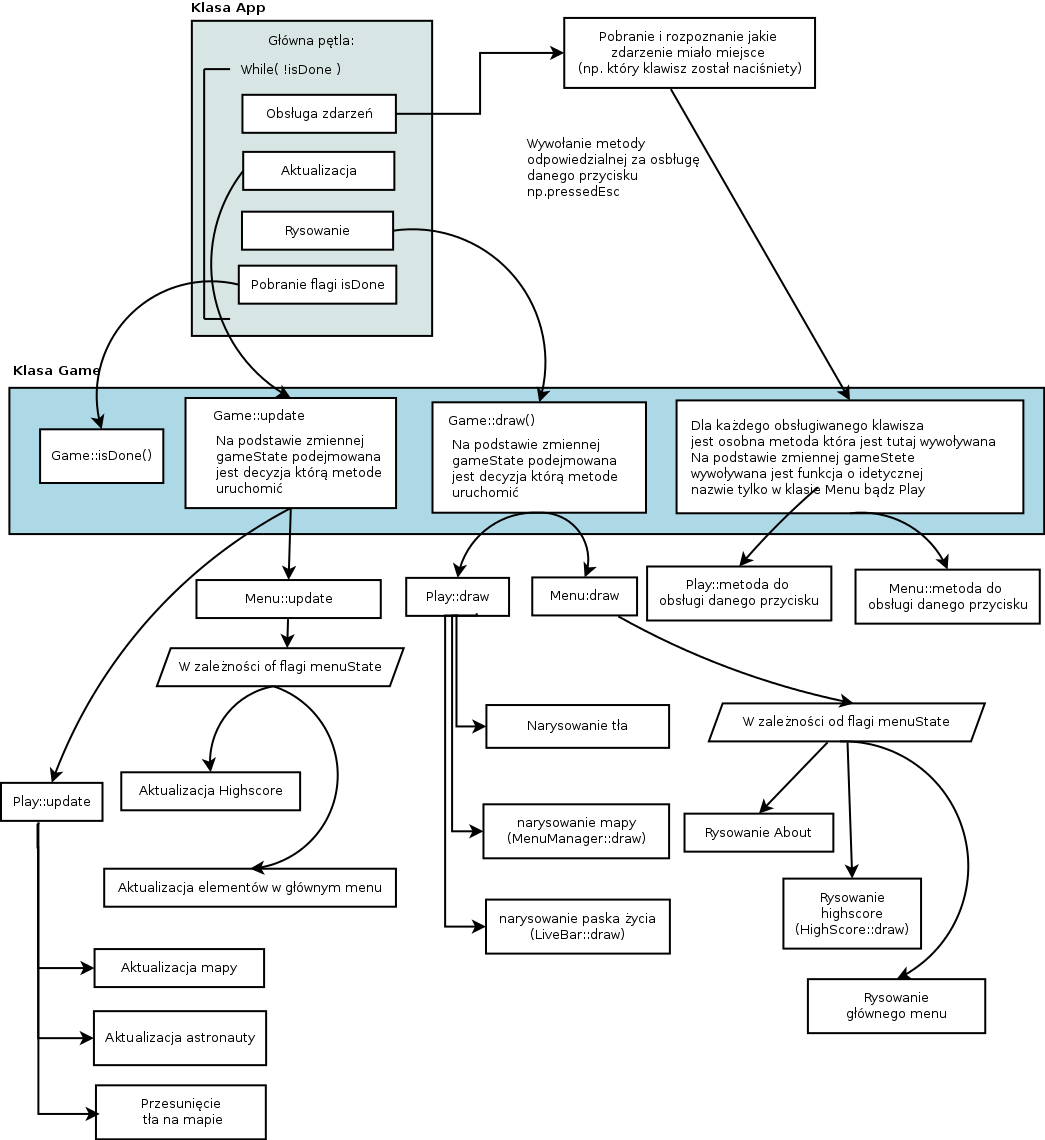
\includegraphics[width=450px,height=630px]{./Pictures/warstwy.png}
    \caption{Schemat przepływu danych w aplikacji}
\end{figure}

\begin{figure}[h]
    \centering
    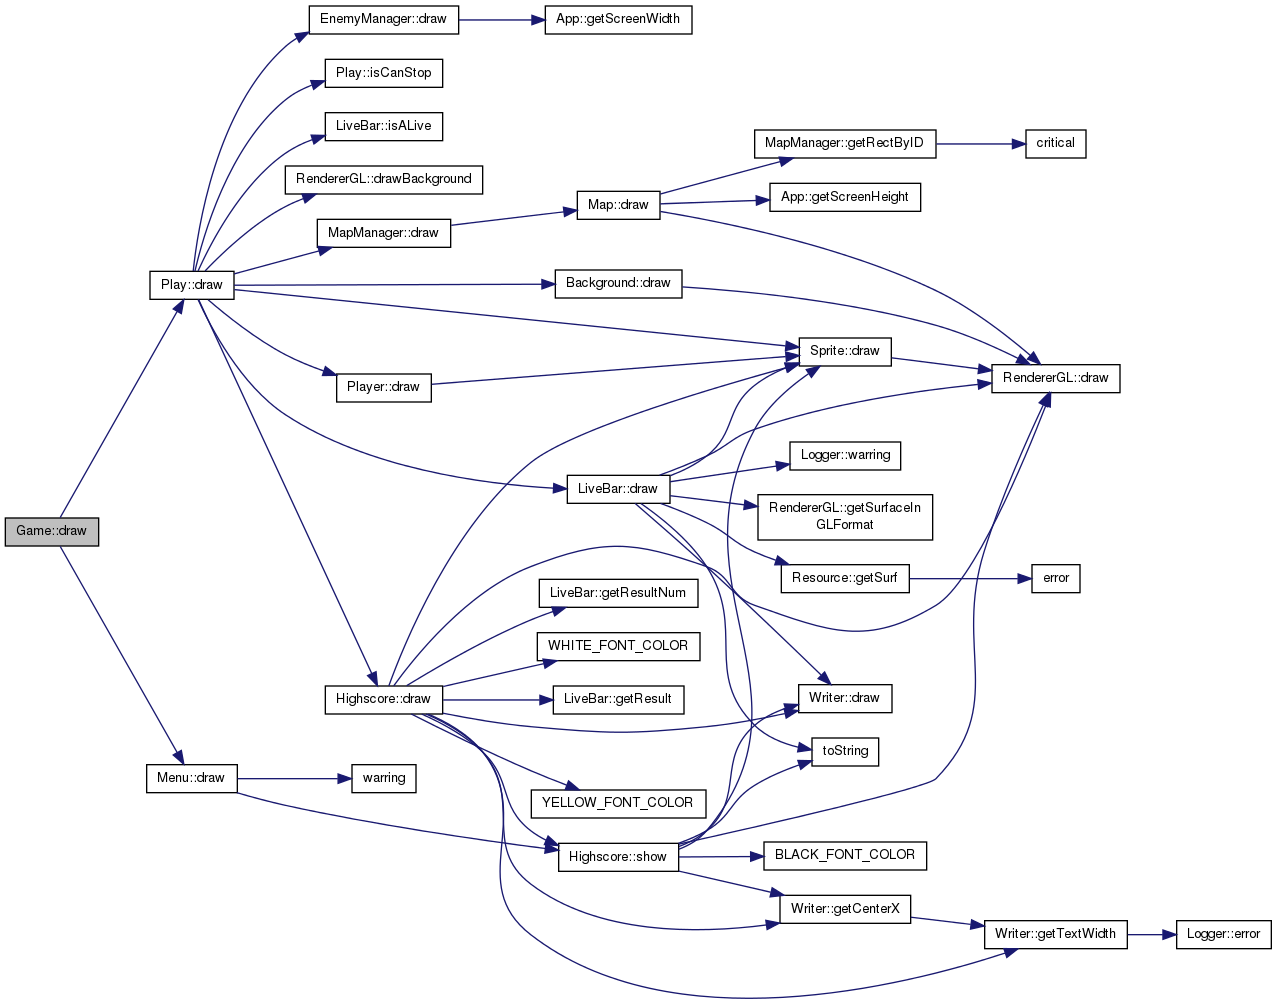
\includegraphics[width=460px,height=550px]{./Pictures/doxygen1.png}
    \caption{Schemat przepływu danych w przypadku wywołania funkcji Game::draw wygenerowany za pomocą programu Doxygen.}
\end{figure}
